\chapter{Thực nghiệm giải quyết 2 bài toán kinh điển}
\section{Thực nghiệm 1: Chia ba một góc bất kỳ}
\subsection{Quy trình}
Phương pháp do Abe Hisashi công bố năm 1980 cho phép chia đều một góc nhọn bất kỳ thành ba phần bằng nhau bằng việc kết hợp các nếp gấp song song và Tiên đề 6.

\textbf{Bước 1: Chuẩn bị góc và hai nếp gấp song song}

Xét một tờ giấy hình vuông cạnh $a$. Đặt góc nhọn cần chia ba $\angle AOB = \theta$ tại đỉnh dưới cùng bên trái $O(0,0)$, với cạnh $OB$ nằm trùng trên mép đáy của tờ giấy.

\begin{enumerate}
    \item Dựng nếp gấp ngang $L_1$ song song với mép đáy $L_0$, cách mép đáy một khoảng cách $d$ tùy ý.
    \item Gập mép đáy $L_0$ đè lên nếp gấp $L_1$ để tạo tiếp nếp gấp ngang thứ hai $L_2$ song song với $L_1$, sao cho khoảng cách giữa $L_1$ và $L_2$ cũng bằng đúng $d$.
    \item Đánh dấu giao điểm của nếp gấp $L_1$ với mép đứng bên trái là điểm $P$.
\end{enumerate}

\begin{figure}[H]
    \centering
    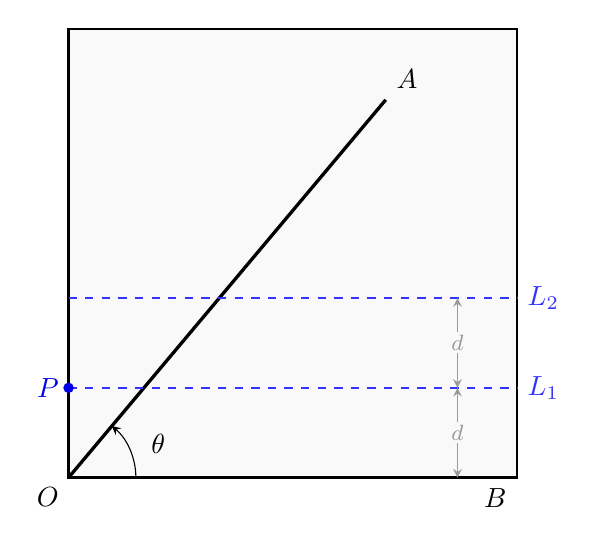
\begin{tikzpicture}[scale=0.95, >=stealth]
        % Tờ giấy vuông
        \draw[thick, fill=gray!5] (0,0) rectangle (6,6);
        \node[below left] at (0,0) {$O$};
        
        % Cạnh góc và tia OA
        \draw[very thick, black] (0,0) -- (6,0) node[below left] {$B$};
        \draw[very thick, black] (0,0) -- (4.24,5.05) node[above right] {$A$};
        \draw[domain=0:50, ->] (0.9,0) arc (0:50:0.9);
        \node at (1.2,0.45) {$\theta$};

        % Hai đường song song L1 và L2
        \draw[thick, blue!80, dashed] (0,1.2) -- (6,1.2) node[right] {$L_1$};
        \draw[thick, blue!80, dashed] (0,2.4) -- (6,2.4) node[right] {$L_2$};

        % Điểm P và các khoảng cách d
        \coordinate (P) at (0,1.2);
        \fill[blue!90!black] (P) circle (2pt) node[left] {$P$};
        
        \draw[<->, gray!80] (5.2, 0) -- (5.2, 1.2) node[midway, fill=gray!5, inner sep=1pt] {\footnotesize $d$};
        \draw[<->, gray!80] (5.2, 1.2) -- (5.2, 2.4) node[midway, fill=gray!5, inner sep=1pt] {\footnotesize $d$};
    \end{tikzpicture}
    \caption{Bước 1: Thiết lập góc $\theta$ tại đỉnh $O$ và dựng hai dải giấy song song cùng bề rộng $d$.}
    \label{fig:abe_step1}
\end{figure}

\textbf{Bước 2: Thao tác mấu chốt theo Tiên đề 6}

Áp dụng Tiên đề 6 cho hệ gồm hai điểm $\{O, P\}$ và hai đường thẳng $\{OA, L_2\}$:
\begin{itemize}
    \item Uốn cong tờ giấy và điều chỉnh duy nhất một nếp gấp $T$ sao cho:
    \begin{itemize}
        \item Đỉnh $O$ thuộc $L_1$
        \item Điểm mấu chốt $P$ tiếp xúc lên $OA$ tại điểm $P'$.
    \end{itemize}
    \item Miết cố định nếp gấp $T$.
\end{itemize}

\begin{figure}[H]
    \centering
    \begin{tikzpicture}[scale=1.05, >=stealth]
        % --- Khung tờ giấy hình vuông Origami ---
        \draw[thick, fill=gray!4] (0,0) rectangle (6,6);
        \coordinate (O) at (0,0);
        \coordinate (B) at (6,0);
        \node[below left, font=\bfseries] at (O) {$O$};
        \node[below left] at (B) {$B$};
        \draw[thick, black] (O) -- (B);

        % --- Hai đường gióng song song L1 và L2 ---
        % L1 ở cao độ y = 1.4, L2 ở cao độ y = 2.8
        \draw[thick, blue!60!black, dashed] (0, 1.4) -- (6, 1.4)
            node[right, font=\footnotesize\bfseries, blue!80!black] {$L_1$};
        \draw[thick, blue!60!black, dashed] (0, 2.8) -- (6, 2.8)
            node[right, font=\footnotesize\bfseries, blue!80!black] {$L_2$};

        % --- Điểm P nằm ở giao của L2 và lề mép trái: (0, 2.8) ---
        \coordinate (P) at (0, 2.8);
        \fill[blue!90!black] (P) circle (2.2pt);
        \node[left, font=\bfseries, blue!90!black] at (P) {$P$};

        % Đỉnh O ban đầu tại góc trái dưới (0,0)
        \fill[black] (O) circle (2.2pt);

        % --- Tia OA (tạo góc theta ~ 50 độ từ gốc O) ---
        \coordinate (A) at (4.2, 5.0);
        \draw[thick, black] (O) -- (A) node[above right] {$A$};

        % --- Nếp gấp Tiên đề 6: T ---
        \coordinate (Fold1) at (0, 4.4);
        \coordinate (Fold2) at (4.6, 0);
        \draw[very thick, teal, dashdotted] (Fold1) -- (Fold2);
        \node[teal!90!black, font=\footnotesize\bfseries, fill=white, inner sep=2pt, draw=teal!40, rounded corners=2pt, rotate=-44] 
            at (3.4, 1.2) {Nếp gấp $T$};

        % --- Các điểm chạm sau khi gập: O' in L1 và P' in OA ---
        % O' nằm chính xác trên L1 (y = 1.4)
        \coordinate (Oprime) at (2.2, 1.4);
        % P' nằm trên đường chứa tia OA
        \coordinate (Pprime) at (2.6, 3.1);

        \fill[red!80!black] (Oprime) circle (2.2pt);
        \node[red!80!black, font=\footnotesize\bfseries, below right, fill=white, inner sep=1.5pt, rounded corners=1pt] 
            at (2.2, 1.3) {$O' \in L_1$};

        \fill[purple!80!black] (Pprime) circle (2.2pt);
        \node[purple!80!black, font=\footnotesize\bfseries, above left, fill=white, inner sep=1.5pt, rounded corners=1pt] 
            at (2.55, 3.25) {$P' \in OA$};

        % --- Mũi tên mô phỏng chuyển động gập ---
        \draw[->, thick, red!80!black, bend right=20] 
            (0.15, 0.1) to node[midway, below right, font=\footnotesize] {gập $O \to L_1$} (2.05, 1.3);

        \draw[->, thick, blue!80!black, bend left=20] 
            (0.15, 2.9) to node[midway, above left, font=\footnotesize] {gập $P \to OA$} (2.45, 3.2);
    \end{tikzpicture}
    \caption{Bước 2: Áp dụng Tiên đề 6 đưa đồng thời đỉnh $O$ chạm vào đường $L_1$ (tại $O'$) và điểm $P$ trên lề đường $L_2$ chạm vào tia $OA$ (tại $P'$) qua nếp gấp $T$.}
    \label{fig:abe_step2}
\end{figure}

   
\textbf{Bước 3: Mở nếp gập và thu nhận ba góc bằng nhau}

Khi mở tờ giấy ra:
\begin{enumerate}
    \item Nếp gấp T cắt $L_1$ tại $K$.
    \item Gấp theo đường thẳng $OK$.
    \item Gấp mép $OB$ trùng với $OK$
    \item Góc $\angle AOB$ ban đầu bị phân chia chính xác thành ba góc bằng nhau:
    \begin{equation}
        \theta_1 = \theta_2 = \theta_3 = \frac{\theta}{3}.
    \end{equation}
\end{enumerate}

\begin{figure}[H]
    \centering
    \begin{tikzpicture}[scale=1.1, >=stealth]
        % --- Khung tờ giấy hình vuông Origami ---
        \draw[thick, fill=gray!4] (0,0) rectangle (6,6);
        \coordinate (O) at (0,0);
        \coordinate (B) at (6,0);
        \node[below left] at (O) {$O$};
        \node[below left] at (B) {$B$};

        % --- Tia OB (cạnh đáy) và tia OA (góc theta = 60 độ) ---
        \coordinate (A) at (60:5.5);
        \draw[thick, black] (O) -- (B);
        \draw[thick, black] (O) -- (A) node[above right] {$A$};

        % --- Hai đường song song L1 và L2 ---
        % L1 ở cao độ d = 1.6
        \draw[thick, blue!50, dashed] (0, 1.6) -- (6, 1.6);
        \node[font=\footnotesize\bfseries, blue!80!black, fill=white, inner sep=1.5pt, rounded corners=1pt] 
            at (5.7, 1.85) {$L_1$};

        % L2 ở cao độ 2d = 3.2
        \draw[thick, blue!50, dashed] (0, 3.2) -- (6, 3.2);
        \node[font=\footnotesize\bfseries, blue!80!black, fill=white, inner sep=1.5pt, rounded corners=1pt] 
            at (5.7, 3.45) {$L_2$};

        % --- Điểm K = T \cap L1: Nằm chính xác trên góc 40 độ tại y = 1.6 ---
        \coordinate (K) at (40:2.489);

        % --- Nếp gấp T ban đầu (đi qua K) ---
        \draw[thick, teal!40, dashdotted] (-0.3, 4.2) -- (4.8, -0.4);
        \node[teal!70!black, font=\scriptsize, fill=white, inner sep=1pt, rounded corners=1pt] 
            at (3.6, 0.6) {Nếp gấp $T$};

        % Điểm K
        \fill[red!80!black] (K) circle (2.2pt);
        \node[red!80!black, font=\footnotesize\bfseries, fill=white, inner sep=1.5pt, rounded corners=1pt] 
            at (1.9, 2.05) {$K = T \cap L_1$};

        % --- 1. Đường OK: Tia chia góc thứ hai (40 độ = 2*theta/3) ---
        \draw[very thick, purple!90!black] (O) -- (40:5.8);
        \node[purple!90!black, font=\footnotesize\bfseries, fill=white, inner sep=2pt, rounded corners=2pt, right] 
            at (40:5.8) {Đường $OK$ $\left(\frac{2\theta}{3}\right)$};

        % --- 2. Đường phân giác khi gập OB -> OK (20 độ = theta/3) ---
        \draw[very thick, orange!90!black, dashed] (O) -- (20:5.8);
        \node[orange!90!black, font=\footnotesize\bfseries, fill=white, inner sep=2pt, rounded corners=2pt, right] 
            at (20:5.8) {Gấp $OB \to OK$ $\left(\frac{\theta}{3}\right)$};

        % --- 3 cung góc hiển thị 3 phần bằng nhau (20 độ mỗi góc) ---
        % Góc 1: [0 -> 20 độ]
        \draw[->, thick, gray!80] (2.2, 0) arc (0:20:2.2);
        \node[font=\footnotesize\bfseries] at (10:2.6) {$\frac{\theta}{3}$};

        % Góc 2: [20 -> 40 độ]
        \draw[->, thick, gray!80] (20:2.2) arc (20:40:2.2);
        \node[font=\footnotesize\bfseries] at (30:2.6) {$\frac{\theta}{3}$};

        % Góc 3: [40 -> 60 độ]
        \draw[->, thick, gray!80] (40:2.2) arc (40:60:2.2);
        \node[font=\footnotesize\bfseries] at (50:2.6) {$\frac{\theta}{3}$};
    \end{tikzpicture}
    \caption{Bước 3: Mở nếp gập, xác định giao điểm $K = T \cap L_1$. Đường $OK$ và đường phân giác khi gập $OB \to OK$ chia góc ban đầu thành ba phần bằng nhau.}
    \label{fig:abe_step3}
\end{figure}

\subsection{Thực nghiệm}
Thực nghiệm làm trên các khổ giấy 15cmx15cm và 20cmx20cm với các góc $\theta=45^\circ$ và $\theta=90^\circ$.
\begin{center}
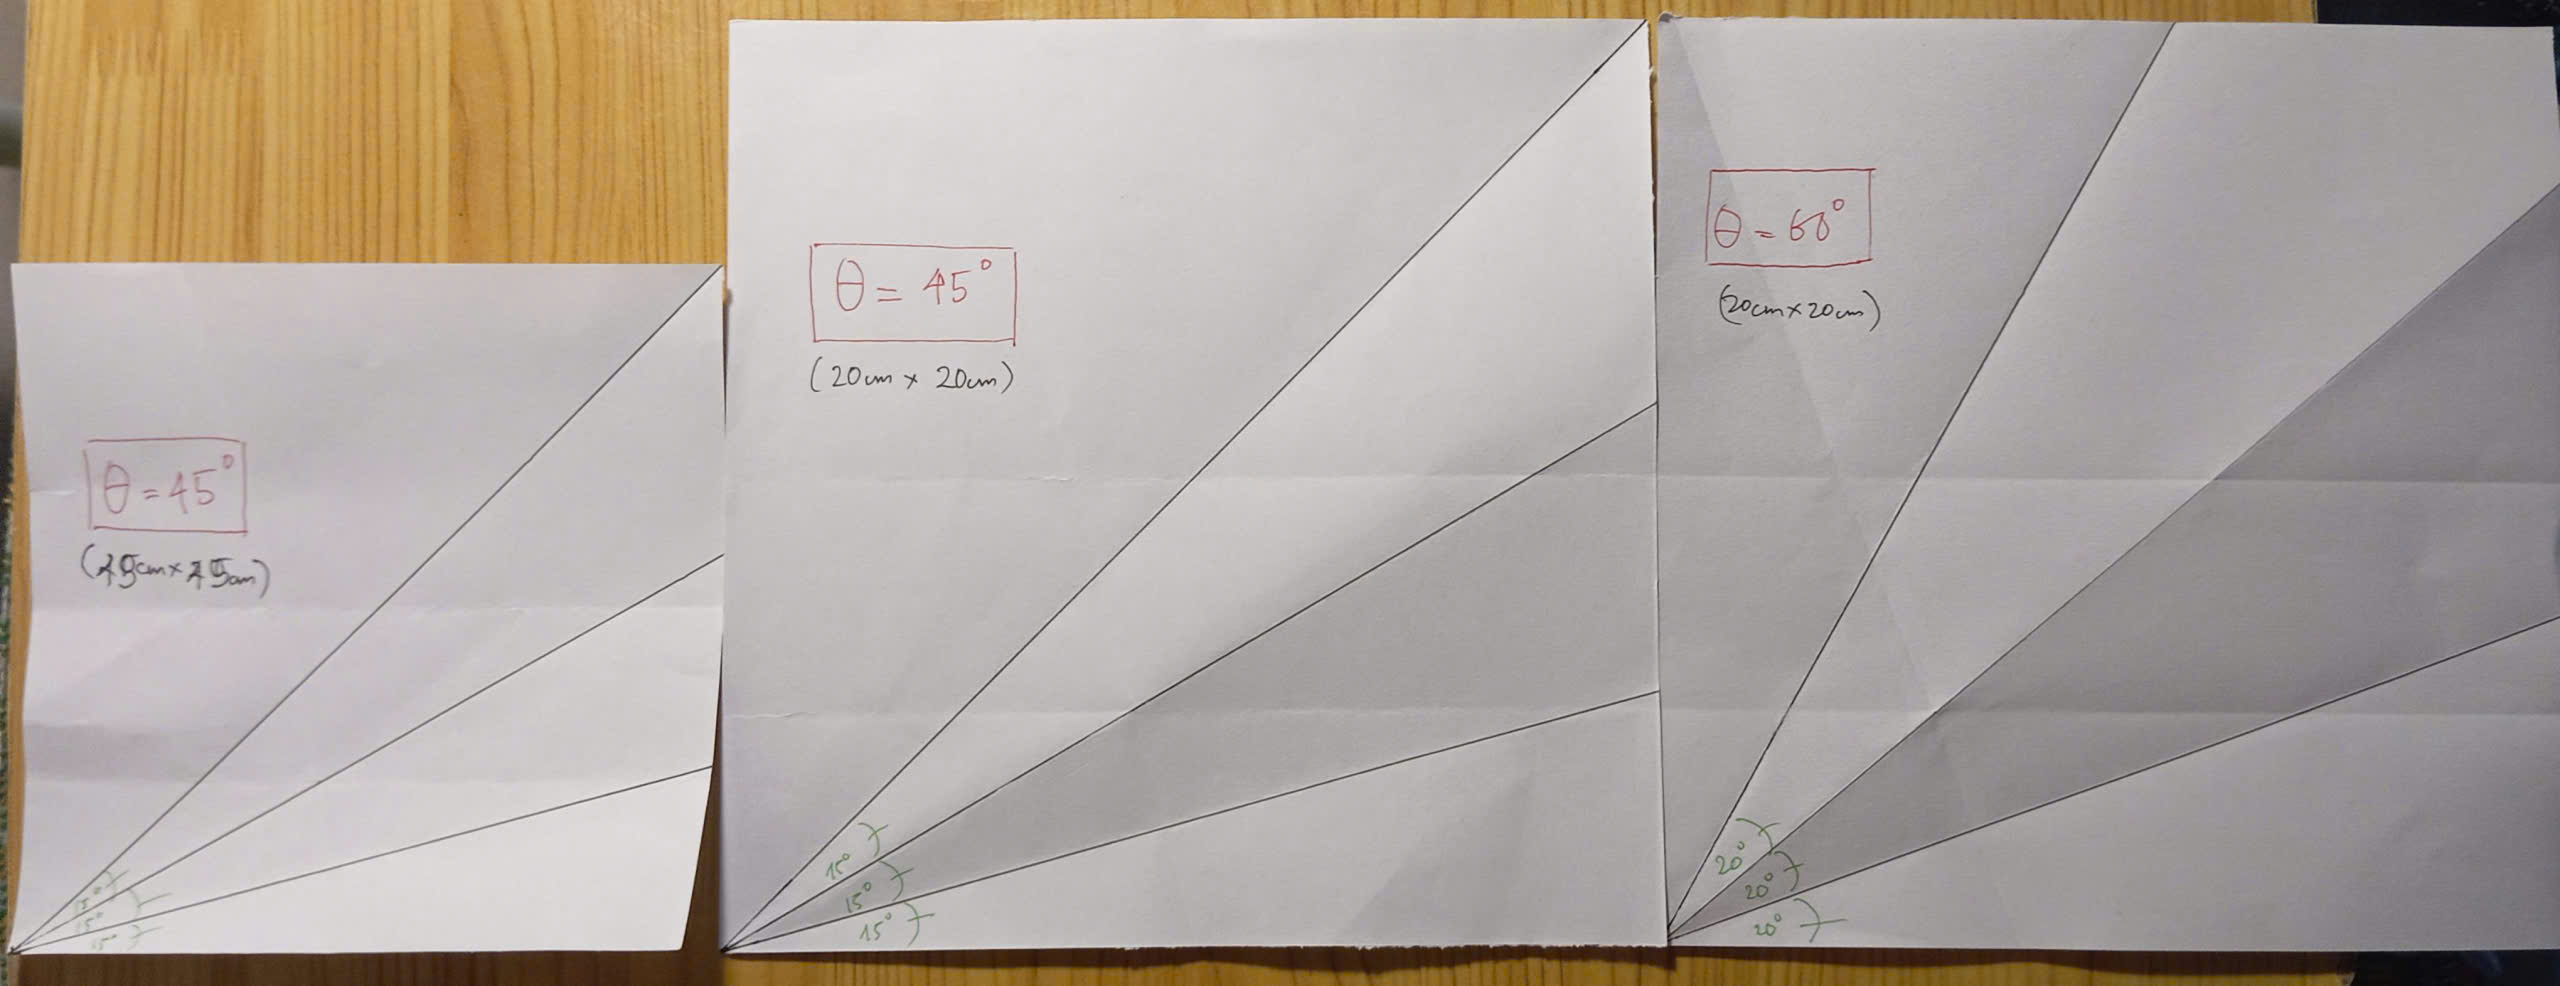
\includegraphics[scale=0.15]{photos/trisectangle.jpg}
\end{center}

\textbf{Nhận xét:} Cách chia này khá chính xác và không thay đổi nếu kích thước khổ giấy 15cmx15cm và 20cmx20cm với góc $\theta=45^\circ$.

\section{Thực nghiệm 2: Dựng tỷ lệ $\sqrt[3]{2}$ (Phương pháp Peter Messer)}

\subsection{Quy trình}
Phương pháp của Peter Messer (1986) cho phép nhân đôi khối lập phương bằng cách xác định tỷ lệ $\sqrt[3]{2}$ trực tiếp trên mép cạnh của tờ giấy hình vuông thông qua Tiên đề 6.

\textbf{Bước 1: Chia tờ giấy thành 3 phần bằng nhau}

Xét tờ giấy hình vuông $ABCD$.
\begin{enumerate}
    \item Chia tờ giấy theo phương ngang thành 3 dải bằng nhau bằng cách ước lượng cuộn mép (hoặc dùng định lý Haga để lấy chính xác tuyệt đối).
    \item Miết tạo hai đường nếp gấp ngang song song: đường nếp dưới $L_1$ và đường nếp trên $L_2$.
\end{enumerate}

\begin{figure}[H]
    \centering
    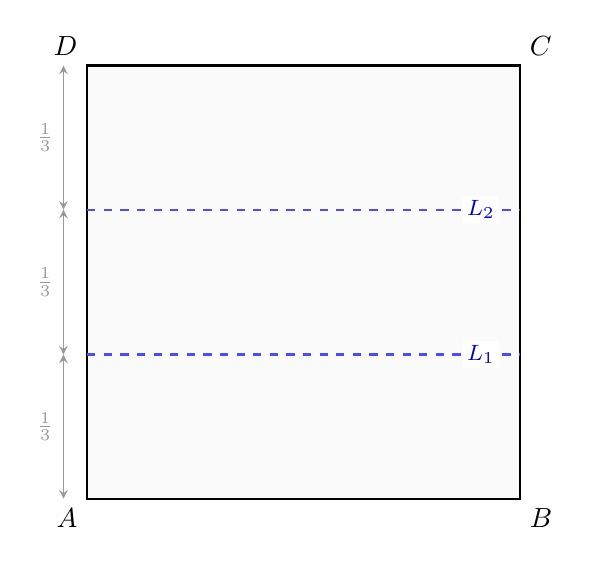
\begin{tikzpicture}[scale=1.0, >=stealth]
        % Tờ giấy vuông ABCD
        \draw[thick, fill=gray!4] (0,0) rectangle (5.5,5.5);
        \node[below left] at (0,0) {$A$};
        \node[below right] at (5.5,0) {$B$};
        \node[above right] at (5.5,5.5) {$C$};
        \node[above left] at (0,5.5) {$D$};

        % Hai nếp gấp chia 3 phần
        \draw[thick, blue!70, dashed] (0, 1.83) -- (5.5, 1.83);
        \node[font=\footnotesize\bfseries, blue!80!black, fill=white, inner sep=1.5pt] at (5.0, 1.83) {$L_1$};

        \draw[thick, blue!70, dashed] (0, 3.67) -- (5.5, 3.67);
        \node[font=\footnotesize\bfseries, blue!80!black, fill=white, inner sep=1.5pt] at (5.0, 3.67) {$L_2$};

        % Đo kích thước 3 phần bằng nhau
        \draw[<->, gray!80] (-0.3, 0) -- (-0.3, 1.83) node[midway, left, font=\footnotesize] {$\frac{1}{3}$};
        \draw[<->, gray!80] (-0.3, 1.83) -- (-0.3, 3.67) node[midway, left, font=\footnotesize] {$\frac{1}{3}$};
        \draw[<->, gray!80] (-0.3, 3.67) -- (-0.3, 5.5) node[midway, left, font=\footnotesize] {$\frac{1}{3}$};
    \end{tikzpicture}
    \caption{Bước 1: Chia tờ giấy thành 3 dải bằng nhau bằng hai nếp gấp ngang $L_1$ (nếp dưới) và $L_2$ (nếp trên).}
    \label{fig:messer_step1}
\end{figure}

\textbf{Bước 2: Nếp gấp Tiên đề 6}

Cầm đỉnh góc dưới bên trái $A$ và thực hiện gập theo Tiên đề 6:
\begin{itemize}
    \item Đưa đỉnh $A$ sang chạm vào mép đứng bên phải $BC$ tại điểm $A'$.
    \item $L_1$ cắt $AD$ tại E. Đưa E chạm vào $L2$ tại $E'$.
    \item Miết cố định nếp gấp chéo $T$ đi qua $E'A'$
\end{itemize}

\begin{figure}[H]
    \centering
    \begin{tikzpicture}[scale=1.05, >=stealth]
        % --- Khung tờ giấy vuông ABCD ---
        \draw[thick, fill=gray!4] (0,0) rectangle (5.5,5.5);
        \coordinate (A) at (0,0);
        \coordinate (B) at (5.5,0);
        \coordinate (C) at (5.5,5.5);
        \coordinate (D) at (0,5.5);
        
        \node[below left] at (A) {$A$};
        \node[below right] at (B) {$B$};
        \node[above right] at (C) {$C$};
        \node[above left] at (D) {$D$};

        % --- Hai nếp gấp ngang song song L1 và L2 ---
        \draw[thick, blue!50, dashed] (0, 1.83) -- (5.5, 1.83) 
            node[pos=0.92, above, font=\footnotesize, blue!80!black] {$L_1$};
        \draw[thick, blue!50, dashed] (0, 3.67) -- (5.5, 3.67) 
            node[pos=0.92, above, font=\footnotesize, blue!80!black] {$L_2$};

        % --- Điểm ban đầu E = L1 \cap AD và đỉnh A ---
        \coordinate (E) at (0, 1.83);
        \fill[blue!90!black] (E) circle (2.2pt);
        \node[blue!90!black, font=\footnotesize\bfseries, left] at (E) {$E$};
        \fill[black] (A) circle (2.2pt);

        % --- Điểm chạm sau khi gập: E' \in L2 và A' \in BC ---
        % E' nằm trên L2 (y = 3.67)
        \coordinate (E_prime) at (3.5, 3.67);
        % A' nằm trên mép đứng BC (x = 5.5, y chia theo tỷ lệ \sqrt[3]{2}: 5.5 / (1 + 1.2599) \approx 2.43)
        \coordinate (A_prime) at (5.5, 2.43);

        % --- Nếp gấp chéo T đi qua E' và A' ---
        % Đường thẳng nối E'(3.5, 3.67) và A'(5.5, 2.43): y - 2.43 = -0.62 (x - 5.5)
        % Cắt mép trên y = 5.5 tại x \approx 0.55; cắt mép đáy y = 0 tại x \approx 9.4 (vẽ kéo dài trong khung giấy)
        \coordinate (FoldTop) at (0.55, 5.5);
        \coordinate (FoldRight) at (5.5, 2.43);
        \draw[very thick, teal, dashdotted] (FoldTop) -- (FoldRight);
        
        \node[teal!90!black, font=\footnotesize\bfseries, fill=white, inner sep=1.5pt, rounded corners=1pt, rotate=-32] 
            at (2.0, 4.8) {Nếp gấp $T$};

        % Đánh dấu các điểm chạm E' và A'
        \fill[purple!90!black] (E_prime) circle (2.2pt);
        \node[purple!90!black, font=\footnotesize\bfseries, above, fill=white, inner sep=1.5pt, rounded corners=1pt] 
            at (3.5, 3.85) {$E' \in L_2$};

        \fill[red!90!black] (A_prime) circle (2.2pt);
        \node[red!80!black, font=\footnotesize\bfseries, right, fill=white, inner sep=1.5pt, rounded corners=1pt] 
            at (A_prime) {$A' \in BC$};

        % --- Mũi tên uốn cong mô phỏng chuyển động gập ---
        % Gập đỉnh A -> A' \in BC
        \draw[->, thick, red!80!black, bend right=20] 
            (0.15, 0.1) to node[midway, below right, font=\footnotesize] {gập $A \to BC$} (5.35, 2.3);

        % Gập điểm E -> E' \in L2
        \draw[->, thick, blue!80!black, bend left=25] 
            (0.15, 1.95) to node[midway, above left, font=\footnotesize] {gập $E \to L_2$} (3.35, 3.65);
    \end{tikzpicture}
    \caption{Bước 2: Gập đỉnh $A$ sang mép $BC$ tại $A'$, đồng thời đưa điểm $E = L_1 \cap AD$ chạm vào $L_2$ tại $E'$. Nếp gấp $T$ đi qua hai điểm $E'$ và $A'$.}
    \label{fig:messer_step2}
\end{figure}

\textbf{Bước 3: Thu nhận tỷ lệ $\sqrt[3]{2}$ trên mép phải}

Nếu quy ước độ dài đoạn phía dưới $BA'$ làm đơn vị ($1$), thì độ dài đoạn phía trên $A'C$ chính xác bằng căn bậc ba của 2:
\begin{equation}
    \frac{A'C}{BA'} = \sqrt[3]{2} \approx 1{,}25992.
\end{equation}

\begin{figure}[H]
    \centering
    \begin{tikzpicture}[scale=1.0, >=stealth]
        % Tờ giấy vuông ABCD
        \draw[thick, fill=gray!4] (0,0) rectangle (5.5,5.5);
        \node[below left] at (0,0) {$A$};
        \node[below right] at (5.5,0) {$B$};
        \node[above right] at (5.5,5.5) {$C$};
        \node[above left] at (0,5.5) {$D$};

        % Điểm A' trên mép phải
        \coordinate (A_prime) at (5.5, 2.43);
        \fill[red!80!black] (A_prime) circle (2.2pt);
        \node[red!80!black, font=\footnotesize\bfseries, left] at (A_prime) {$A'$};

        % Làm nổi bật 2 đoạn thẳng trên mép phải BC
        % Đoạn dưới: BA' (độ dài 1)
        \draw[line width=2.5pt, blue!80!black] (5.5, 0) -- (A_prime);
        \draw[<->, thick, blue!80!black] (6.0, 0) -- (6.0, 2.43) 
            node[midway, right, font=\small\bfseries] {Đoạn dưới $= 1$};

        % Đoạn trên: A'C (độ dài \sqrt[3]{2})
        \draw[line width=2.5pt, red!80!black] (A_prime) -- (5.5, 5.5);
        \draw[<->, thick, red!80!black] (6.0, 2.43) -- (6.0, 5.5) 
            node[midway, right, font=\small\bfseries] {Đoạn trên $= \sqrt[3]{2} \approx 1{,}2599$};

        % Đường nếp gấp mở mờ để tham chiếu
        \draw[dashed, gray!40] (1.2, 0) -- (5.5, 4.4);
    \end{tikzpicture}
    \caption{Bước 3: Điểm $A'$ chia mép phải của tờ giấy theo đúng tỷ lệ nhân đôi khối lập phương: $\frac{A'C}{BA'} = \sqrt[3]{2}$.}
    \label{fig:messer_step3}
\end{figure}

\subsection{Thực nghiệm}

Thực nghiệm với các khổ giấy 9cmx9cm, 15cmx15cm và 20cmx20cm.
\begin{center}
\includegraphics[scale=0.15]{photos/doublecube.jpg}
\end{center}
\begin{table}[H]
    \centering
    \caption{đo đạc tỉ lệ $A'C / BA'$ theo kích thước giấy}
    \label{tab:paper_size_ratio}
    \small
    \setlength{\tabcolsep}{6pt}
    \renewcommand{\arraystretch}{1.25}
    \begin{tabularx}{\textwidth}{|>{\centering\arraybackslash}m{3.2cm}|>{\centering\arraybackslash}X|>{\centering\arraybackslash}X|>{\centering\arraybackslash}m{2.5cm}|}
        \hline
        \multirow{2}{=}{\centering\textbf{Kích thước giấy}} & \multicolumn{2}{c|}{\textbf{Tỉ lệ $A'C/BA'$ (Phần trên/Phần dưới)}} & \multirow{2}{=}{\centering\textbf{Sai số}} \\
        \cline{2-3}
        & \textbf{Lý thuyết} & \textbf{Thực tế} & \\
        \hline
        $9 \times 9$ & $1.26$ & $1.143$ & $0.117$ \\
        \hline
        $15 \times 15$ & $1.26$ & $1.239$ & $0.021$ \\
        \hline
        $20 \times 20$ & $1.26$ & $1.247$ & $0.013$ \\
        \hline
    \end{tabularx}
\end{table}

\textbf{Nhận xét:} 
\begin{itemize}
  \item Kết quả tương đối chính xác.
  \item Kết quả của khổ 20cmx20cm chính xác hơn khổ 15cmx15cm. Kết quả của khổ 15cmx15cm tốt hơn 9cmx9cm.
\end{itemize}